% !TEX root = main.tex

\subsection{Embodied Energy Inventory and Assumptions}

The main topic of the present analysis is the production, operation and disposal of an Adaptive Solar Facade (ASF). The ASF is composed of six sub-product systems described in Figure \ref{fig:subsystem}. This consists of a CIGS PV panels mounted on an actuator, supported by a cantilever that offsets it from a cable net supporting structure \ref{fig:explodedView}.

\begin{figure}[H]
\begin{center}
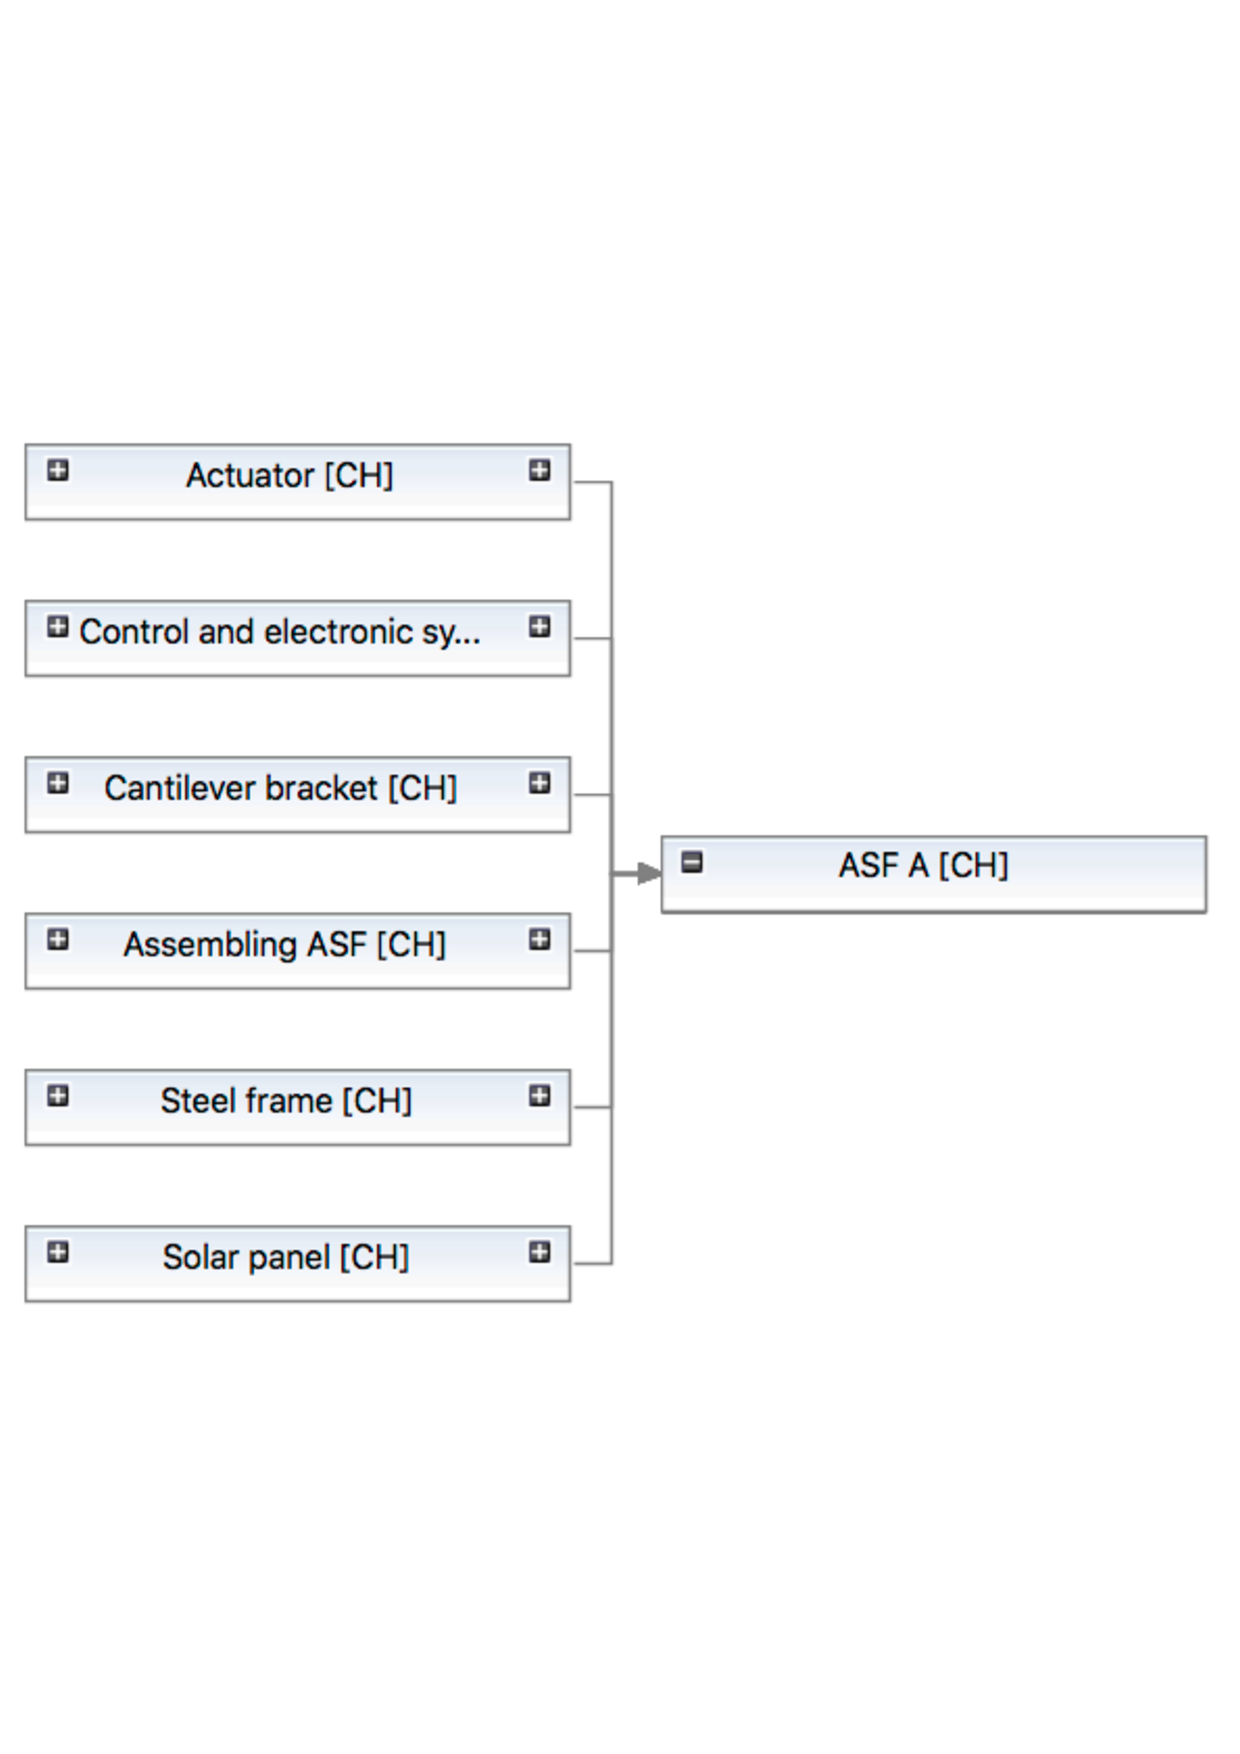
\includegraphics[width=8cm, trim= 0cm 0cm 0cm 0cm,clip]{ASFSubsystems.pdf}
\caption{Breakdown of the ASF into six sub-product systems (Note change Steel frame to Suporting Structure, and Assembling ASF to Assembly. Also redraw this chart so it matches the subsubsections below)}
\label{fig:subsystem}
\end{center}
\end{figure}

\begin{figure}[H]
\begin{center}
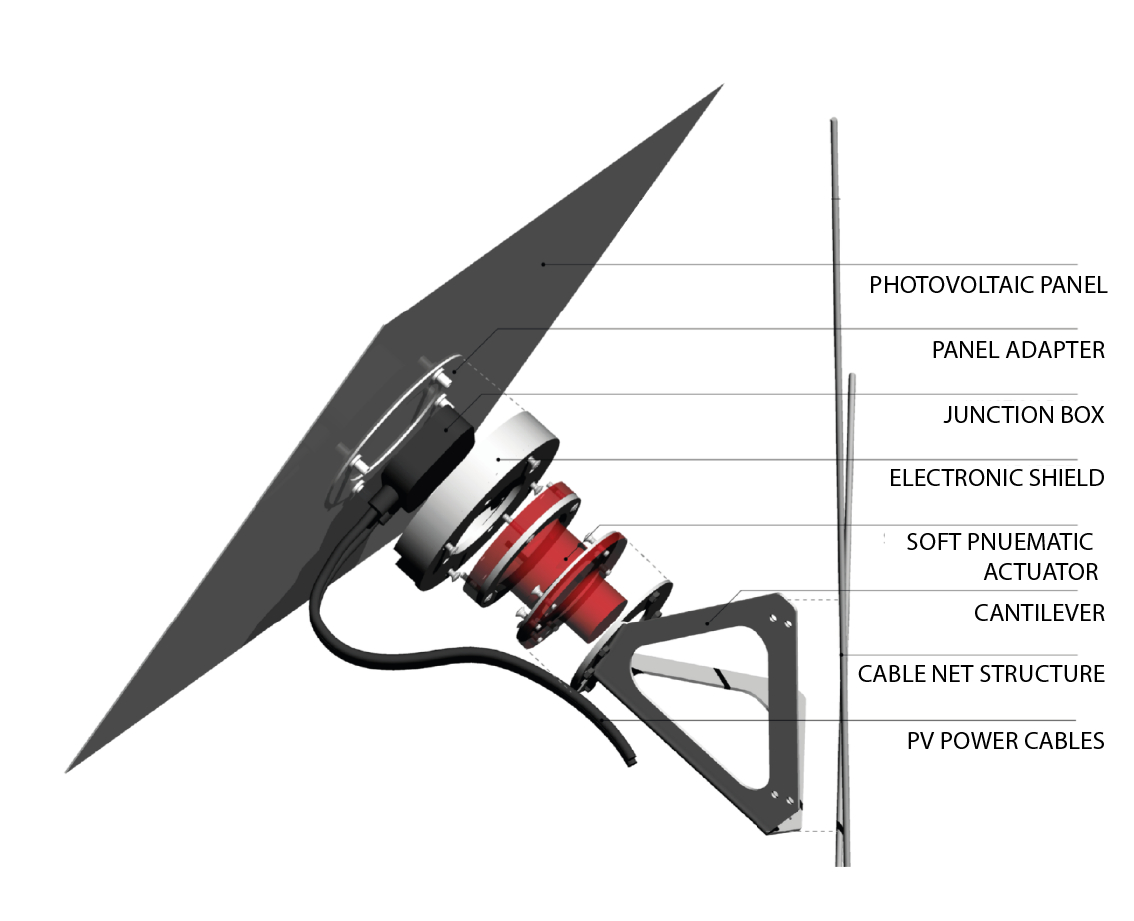
\includegraphics[width=8cm, trim= 0cm 0cm 0cm 0cm,clip]{explodedASFV2.png}
\caption{Exploded view of an ASF module mounted on a cable net supporting structure}
\label{fig:explodedView}
\end{center}
\end{figure}

\subsubsection*{PV Panel}
A CIGS PV panel was selected as the thin film panel of choice due to its high efficiency, low cost, and ability to be mounted on a polymer or aluminium substrate \cite{chirilua2011highly}.\\

The nominal conversion efficiencies are XX\% for teh CIGS panels based off [reference required]\\

[Also make a note about where the PV data comes from, maybe also analyse a-Si?]\\

[Add Inventory Analysis of PV panels here]

\subsubsection*{Actuator}
Traditionally photovoltaic actuation is done through the use of servo motors. Servo motors however become a limiting factor for adaptive facades due to their high upfront costs, and instability to heavy winds. Soft robotic actuators on the other hand are cheaper and more resilient to environmental conditions\cite{Svetozarevic2014a}. For the purpose of this analysis we will analyse both servo motors and soft robotic actuators. \\

[Add Inventory Analysis of actuators here, note I would move the air compressor to the actuator section ]

\subsubsection*{Cantilever}
The cantilever is a steel connection point between the PV panel and the supporting structure.\\

[Add Inventory Analysis of cantilever here]

\subsubsection*{Supporting Structure}
The supporting structure is the connection point between the array of photovoltaic modules and the building itself. The design currently in use consists of a steel cable-net that spans a steel supporting frame. The steel frame is then attached to the building itself.\\

[Add Inventory Analysis of supporting structure here]

\subsubsection*{Controls and Electronic System}
The control system is required for the actuation of panels and the regulation of photovoltaic electricity production.\\

[Add Inventory Analysis of control system here]

\subsubsection*{Installation}

The installation of the ASF to the building requires a hydraulic hoist which needs to be in operation for eight hours based off our construction experience \cite{jayathissa2015abs}. \\

[Add Inventory analysis of installtion]


\subsection{Operational Emissions and Assumptions}

The potential savings are based off previously completed numerical simulation \cite{jayathissa2015abs}. The simulation was conducted on a south facing office room. The room xx meters in length, xx meters wide and xx meters high was modeled using Rhinoceros 3D CAD Package \cite{Rhino}, shown in Figure XX. Grasshopper \cite{grasshopper} was used to model the dynamic aspects of the ASF which consists of an array of 400mm CIGS solar panels. The geometrical input is imported to Energy Plus \cite{energyplus} though the DIVA \cite{DIVA} interface. A single zone thermal analysis was conducted for each possible geometrical configuration of the ASF for each hour of the year. The results were then post processed in Python \cite{python} with the NumPy \cite{numpy}, and pandas \cite{pandas} plug-ins. \\

Based on the assumption of XX full openings and closings per day, we approximate the energy requirement to actuate the ASF to be YY kWh in its lifetime.\\

[Table of simulation parameters, and render of Rhino model]


\subsection{Analysis of Reference Cases}

There are two reference cases used for technological comparisons. Firstly the....


\subsection{LCA Methodology}



\begin{itemize}
\item The analysis is performed according to ISO 14040, ISO 14044 and ISO 15804. % 15804 to be discussed
	\item The impact category, which will be evaluated, is the global warming potential (GWP). This is described as the emissions of ${\mathrm{CO_2-eq}}$ in kilograms divided by the functional unit.
	\item The functional unit used is twofold and based on the function of the adaptive building envelope. For the comparison with other shading systems facade area in ${\mathrm{m^2}}$ is used, while comparison with other photovoltaic systems is done using electricity produced in ${\mathrm{kWh}}$. According to the guidelines of the International Energy Agency (IEA), the calculation of kWh produced needs to be based for consistency on conversion efficiency ${\eta}$, performance ratio PR, irradiation I, lifetime LT and area A of the module. Equation \ref{eq:solar} gives the exact formulation:
	% Variables in italics?
	% LT - service life?
\begin{equation}
G=\frac{{\mathrm{GWP}}}{{\mathrm{I \cdot \eta  \cdot PR \cdot LT \cdot A}}}
% what is G
\label{eq:solar}
\end{equation}

	\item The LCI inventory was obtained through...

	\item The scope of the LCA comprises the embodied, operational and disposal global warming impact of the respective system. Figure \ref{fig:BOS} illustrates the system boundaries of the process flows. The supporting structures are also included in the system boundaries. The reason for this is that technologies within the building envelope also change the design of the supporting structures. The supporting structure of solar panels is referred to as balance of systems (BOS).
% We will need to describe a little more what is included and what is not, i.e.
%   not only supporting structure

\begin{figure}[H]
\begin{center}
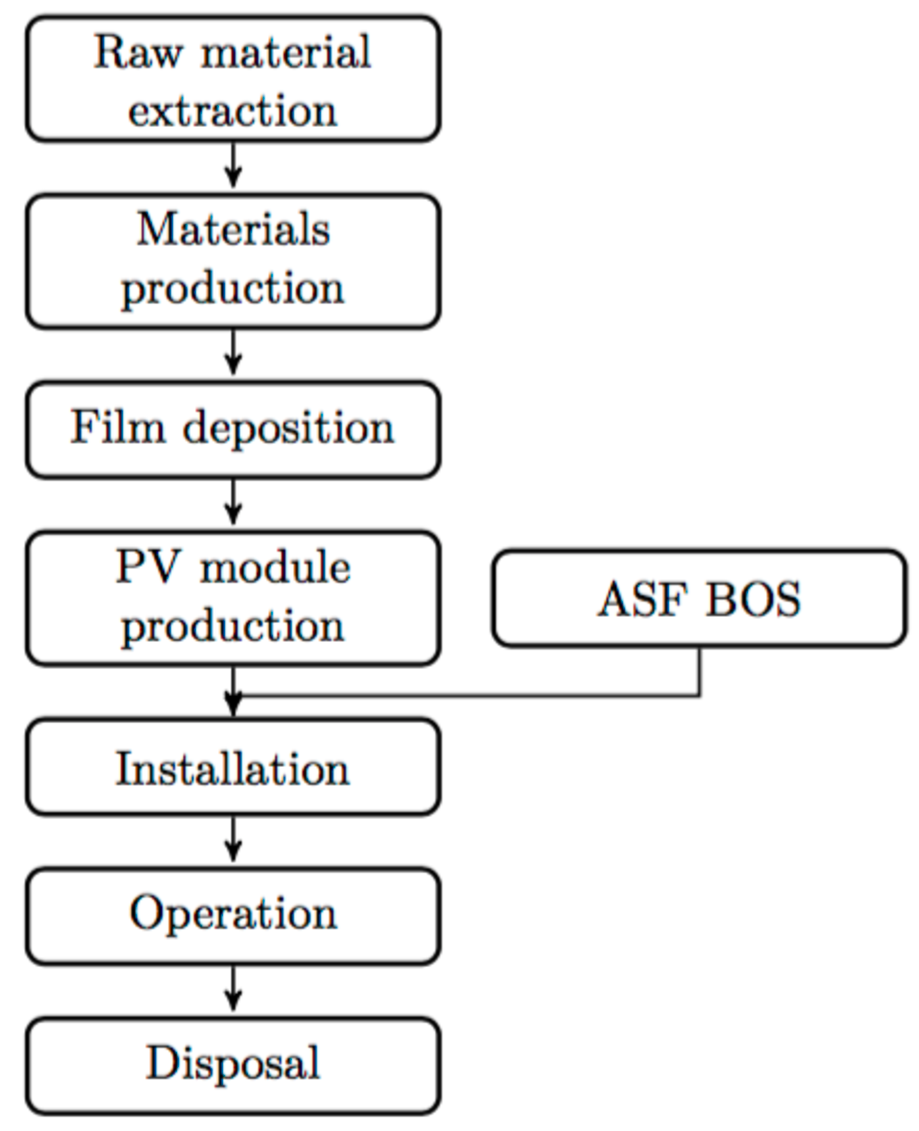
\includegraphics[width=5cm, trim= 0cm 0cm 0cm 0cm,clip]{BOS}
\caption{Thin-film incl. BOS system boundaries}
\label{fig:BOS}
\end{center}
\end{figure}

	\item The cut-off approach is used for recycling and landfill. This means that recycling does not generate any credit for the product and resulting benefits are not taken into account. Furthermore the use of recycled products do not bear the burden of processes higher up the chain.
	% we may need to discuss system expansion
	% PV electricity production not included?
	\item The recipe midpoint (H) allocation method allows for an accurate evaluation of the GWP based on human impact factors.
	% I don't get it - sorry
	% I am pretty sure ReciPe basically uses the IPCC method
\end{itemize}



% what LCI DB (ecoinvent) is used? refer to Annex?
% How was LCI data collected?
% see above. Explain what is included and excluded
